
% JJ

%%%%%%%%%
%
% Subsection: Timing Testing
%
%%%%%%%%%

\subsection{Timing Testing}


\begin{tabular}{r r r r r}
 & \multicolumn{4}{c}{\textbf{Execution times (seconds)}} \\
\textbf{Total Lines} & \underline{32 Cores} & \underline{64 Cores} & \underline{128 Cores} & \underline{200 Cores} \\
       50,000 &   0.55 &     0.57 &     15.49 & 15.45 \\
      500,000 &   4.18 &     5.51 &      4.06 & 9.18 \\
   5,000,0000 &  39.49 &    50.01 &           & 65.05 \\
   50,000,000 & 234.73 &   404.49 &           & 574.71 \\
  500,000,000 &        & 2,094.11 &  3,685.35 & \\
1,000,000,000 &        & 4,146.69 &           &  \\
2,000,000,000 &        &          &           & 21,355.30 \\ 
\end{tabular}

\begin{figure}
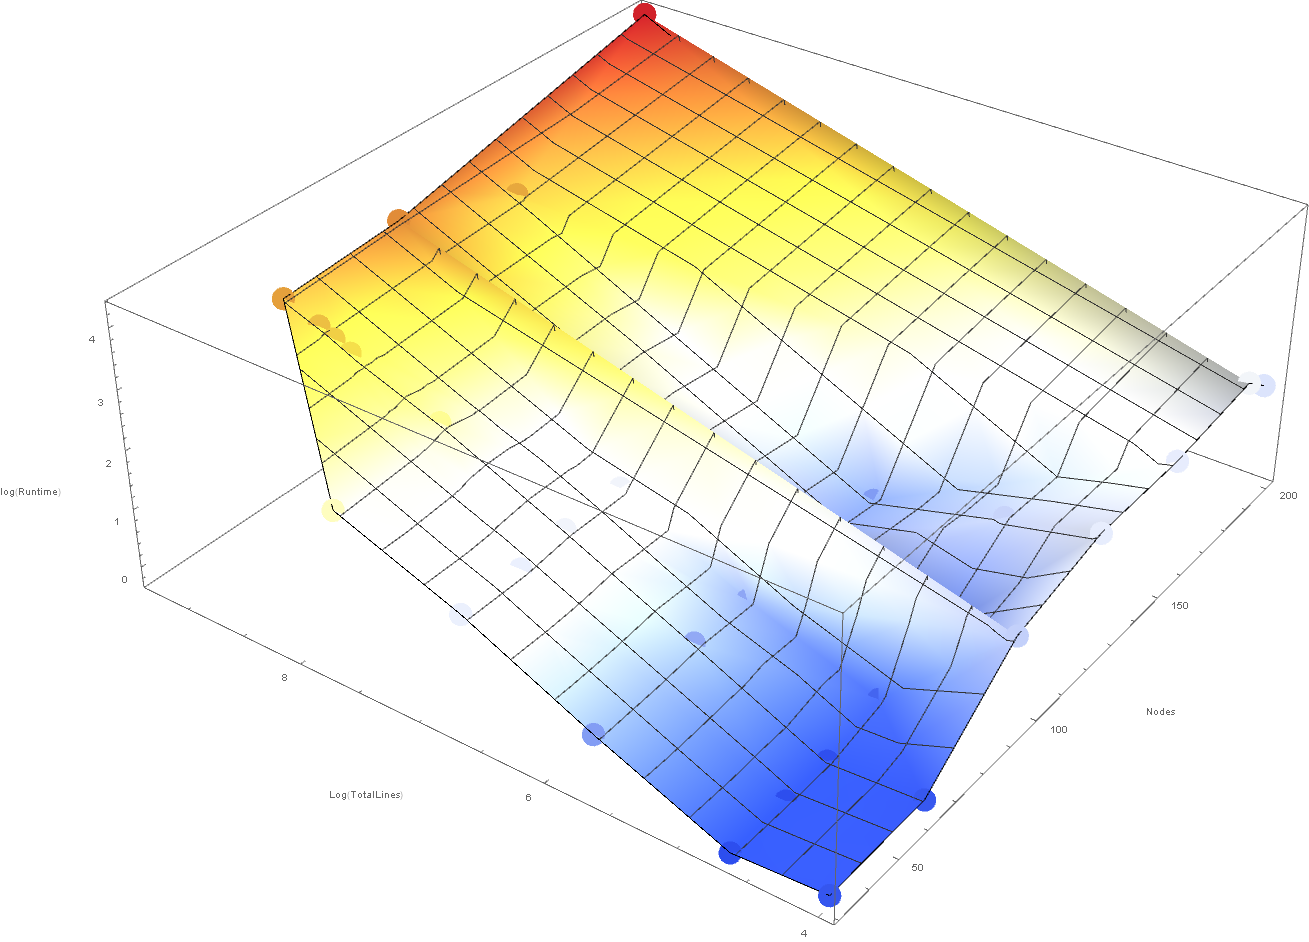
\includegraphics[width=0.9\textwidth]{./images/runtimes.png}
\caption{Execution time versus nodes and total lines}
\end{figure}


\begin{figure}
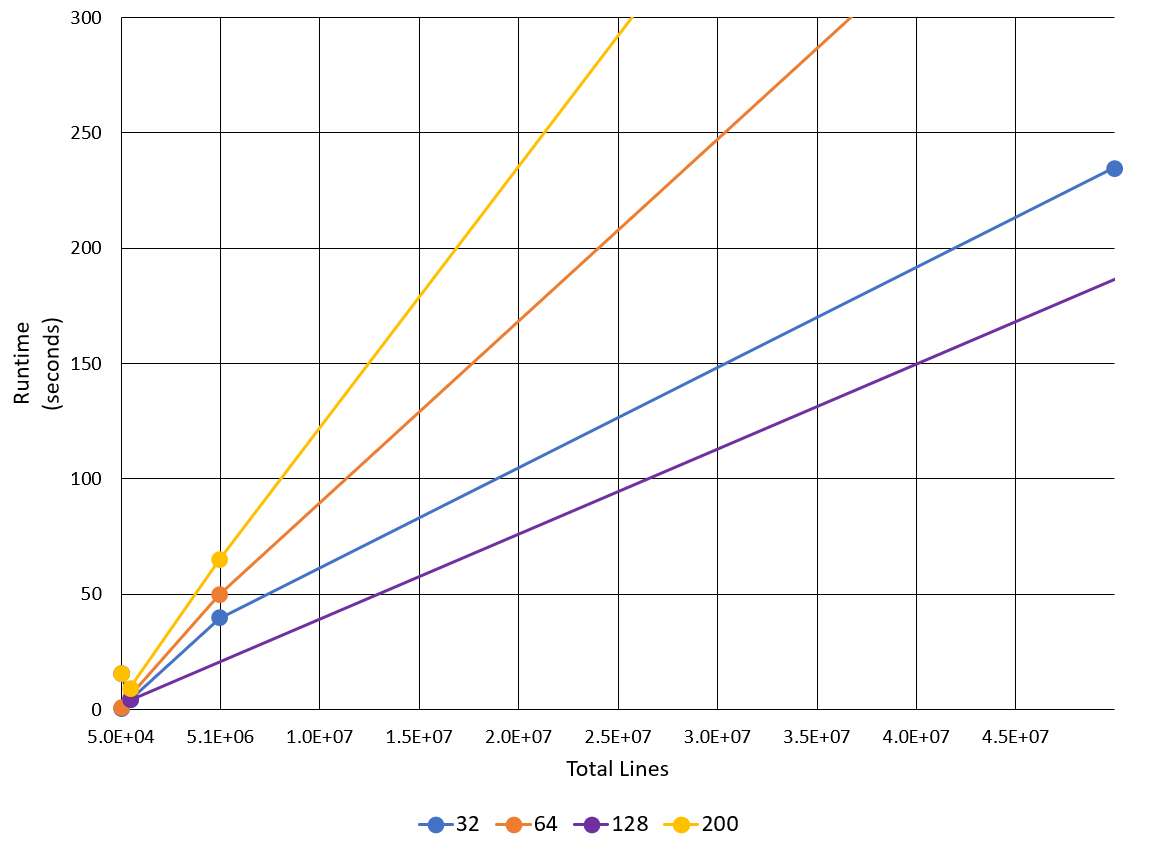
\includegraphics[width=0.9\textwidth]{./images/Runtime1.png}
\caption{Execution time versus nodes for total lines from 50,000 to 50,000,000}
\end{figure}


\begin{figure}
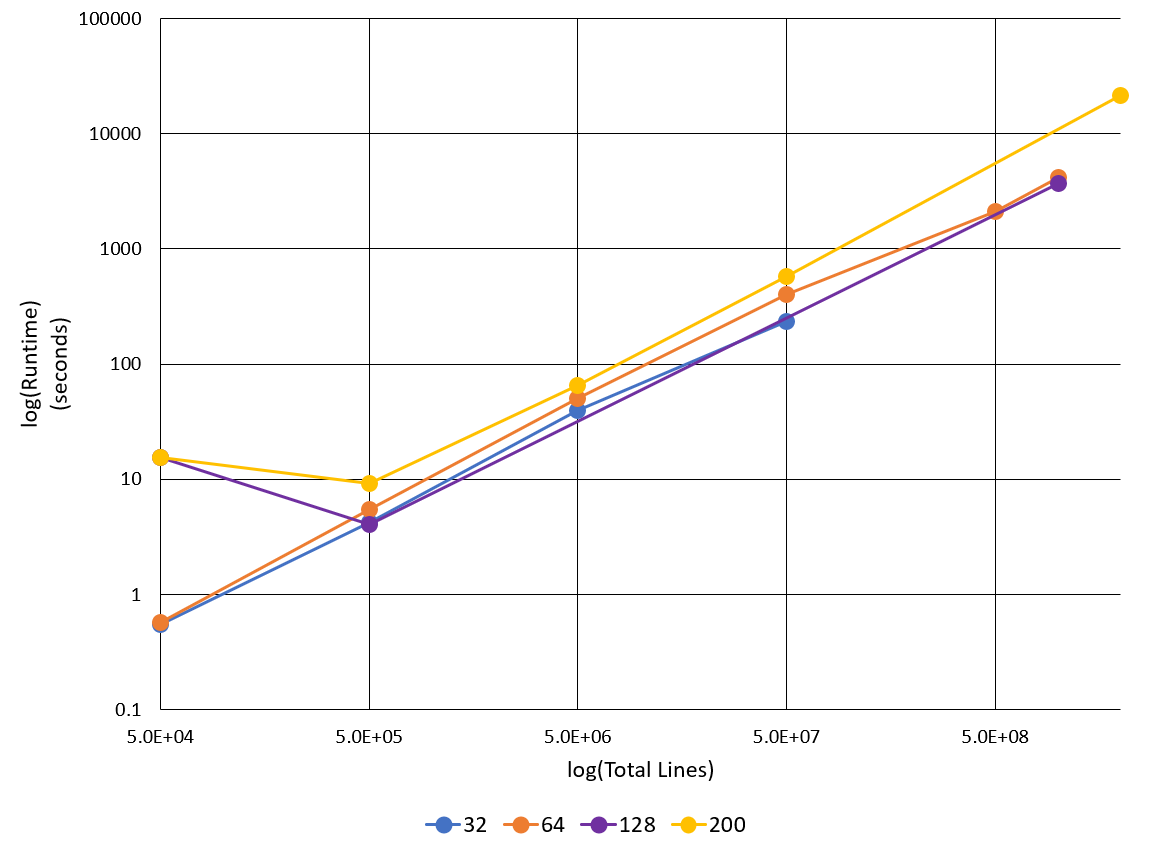
\includegraphics[width=0.9\textwidth]{./images/Runtime2.png}
\caption{Execution time versus nodes and total lines}
\end{figure}

\begin{figure}
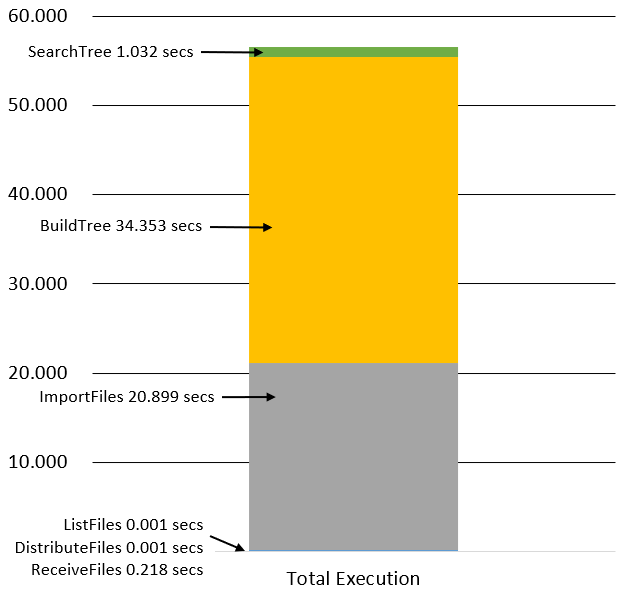
\includegraphics[width=0.9\textwidth]{./images/Runtime3.png}
\caption{Execution time by function for 5,000,000 total lines and 1,000 search rows}
\end{figure}


%%%%%%%%%
%
% Subsection: Search Results
%
%%%%%%%%%

\subsection{Search Results}

The program exports a table at the end of the run displaying the number of points contained in each of three radii centered at each row of points from  \texttt{datafile00501.txt}. The first twenty rows of the output are shown below:

\begin{verbatim}
POINTS FOUND:
 X             Y             Z                   0.01          0.05          0.10
------------  ------------  ------------  ------------  ------------  ------------
    0.581959      0.721012      0.969341        917205      55498018      92120227
    0.894312      0.362959      0.447526         13375       1634169      12135389
    0.801765     -0.037433      0.616920          4026        490535       3837163
    0.685972      0.346683      0.388596         29251       3420777      22785611
    0.716828      0.953059      0.275552          3771        462728       3675457
    0.113410      0.650905      0.795308        797814      53199022      78642100
    0.125404      0.282296      0.536048          1473        187628       1556214
    0.557424      0.471667     -0.075745          1559        190467       1523646
    0.557737      0.697675      0.934643        819217      52896281      92109359
    0.353073      0.840097     -0.000039          1631        195440       1564030
    0.365097      0.064303      0.803032         13811       1693414      12855261
    0.917744      0.511031      1.053122        180759      18109472      67214583
    0.611690     -0.057995      0.263766          1519        186829       1523365
    0.302634      0.128243      0.582824         13350       1586273      11476583
    0.081476     -0.081441      0.254356       2146813      64790807      70678329
    0.215516      0.171119      0.695714          5494        713031       5878422
    0.783198      0.920994      0.874636          2626        317146       2514096
    1.057458      0.734861      0.620092          2985        357166       2338251
    0.399678     -0.069887      0.666980         12781       1560145      11866273
    0.823353      0.852015     -0.053596          3058        371959       2943893
\end{verbatim}

The program was tested using 
